Los procesos de simulación de física de altas energías posee muchas desventajas, entre ellas están los altos requerimientos computacionales para generar las simulaciones y para guardar los resultados, por lo que se hace necesario para la investigación el uso de poderosas supercomputadoras como el \textbf{ACARUS}(\textbf{Á}rea de \textbf{C}ómputo de \textbf{A}lto \textbf{R}endimiento de la \textbf{U}niversidad de \textbf{S}onora), recurso dedicado a la investigación de los cuerpos académicos de la universidad.

\subsubsection{Configuración e implementación de recursos en ACARUS.}
El recurso a usar es el cluster \url{ocotillo.acarus.uson.mx} con un IP \url{148.225.111.150}, este debe ser debidamente configurado con las herramientas necesarias para el proceso de generación. Se hace necesario una sección autorizada en el servidor, y seguir los pasos de conexión específicados en el portal del proyecto \url{http://acarus.uson.mx/clusters/guia.htm}, todo el trabajo se realiza por medio de una terminal, cuestión que imposibilita el uso del recurso sin conocimientos previos de Linux.

Los programas \textbf{ROOT} (sección \ref{C_root}), \textbf{Madgraph} (sección \ref{C_madgraph}), \textbf{Delphes} (sección \ref{C_delphes}) y \textbf{pythia8} (sección \ref{C_pythia8}) deben ser integradas debidamente para correr de forma seriada, el procedimiento de instalación y configuración se pueden encontrar en \url{https://twiki.cern.ch/twiki/bin/view/CMSPublic/MadgraphTutorial}. 

\subsubsection{Gestión de recursos con Slurm.}

Además el sistema gestiona el uso de los recursos entre sus usuarios mediante un sistema de gestión de tareas y de clústeres \href{https://es.wikipedia.org/wiki/Simple\_Linux\_Utility\_for\_Resource\_Management}{\textbf{Slurm}} (\textbf{S}imple \textbf{L}inux \textbf{U}tility for \textbf{R}esources \textbf{M}anagement). Esta herramienta posibilita asignar a los usuarios acceso a nodos de cómputo durante un tiempo determinado, proporciona un framework que permite iniciar, ejecutar y supervisar el trabajo y además se encarga de arbitrar la necesidad de recursos, administrando una cola de tareas pendiente. La documentación relativa al uso de esta herramienta se puede encontrar en el enlace de sus desarrolladores \url{https://slurm.schedmd.com/documentation.html}. Para el caso que nos ocupa en nuestra investigación, para poder paralelizar el proyecto de generación desarrollado en python se prepara un fichero (script) con los datos del trabajo a ejecutar y el modo de utilizar de los recursos requeridos, el usado en este proyecto contiene la siguiente configuración:\\[.2cm]
\begin{footnotesize}
\texttt{\begin{tabular}{ll}
\textbf{\#SBATCH }--nodes=4                 & \# Maximo numero de nodos para asignarse\\
\textbf{\#SBATCH} --ntasks-per-node=8          & \# Maximo numero de tareas en cada nodo\\
\textbf{\#SBATCH} --ntasks=40                  & \# Maximo numero de tareas totales\\
\textbf{\#SBATCH} --distribution=cyclic:cyclic & \# Modo de distribucion de tareas\\
\textbf{\#SBATCH }--mem-per-tasks=1000         & \# Memoria asginada por tarea\\
\textbf{\#SBATCH} --mail-type=END              & \# Momento de notificacion\\
\textbf{\#SBATCH} --mail-user=xxx@gmail.com    & \# Correo a notificar\\
\textbf{\#SBATCH} --job-name=DarkSUSY          & \# Nombre del trabajo                                                                                                                         \\
\textbf{\#SBATCH} --time=168:0:0               & \# Tiempo maximo de ejecucion                                                                                                                                   \\   
\textbf{\#SBATCH} --partition=general          & \# Nombre de la particion                                                                                                                                    \\
\textbf{\#SBATCH} --constraint=broadwell                                                                                                                                 \\
\textbf{srun} python genera\_v5.py & \\
\end{tabular}}
\end{footnotesize}\\[.2cm]

El código anterior gestiona los recursos del crúster para que se ejecute en paralelo el programa generador \texttt{genera\_v5.py} siento este el desarrollado para generar las muestras que se precisan para la investigación.

\subsubsection{Proyecto de python generador.}
\begin{figure}[h]
\centering
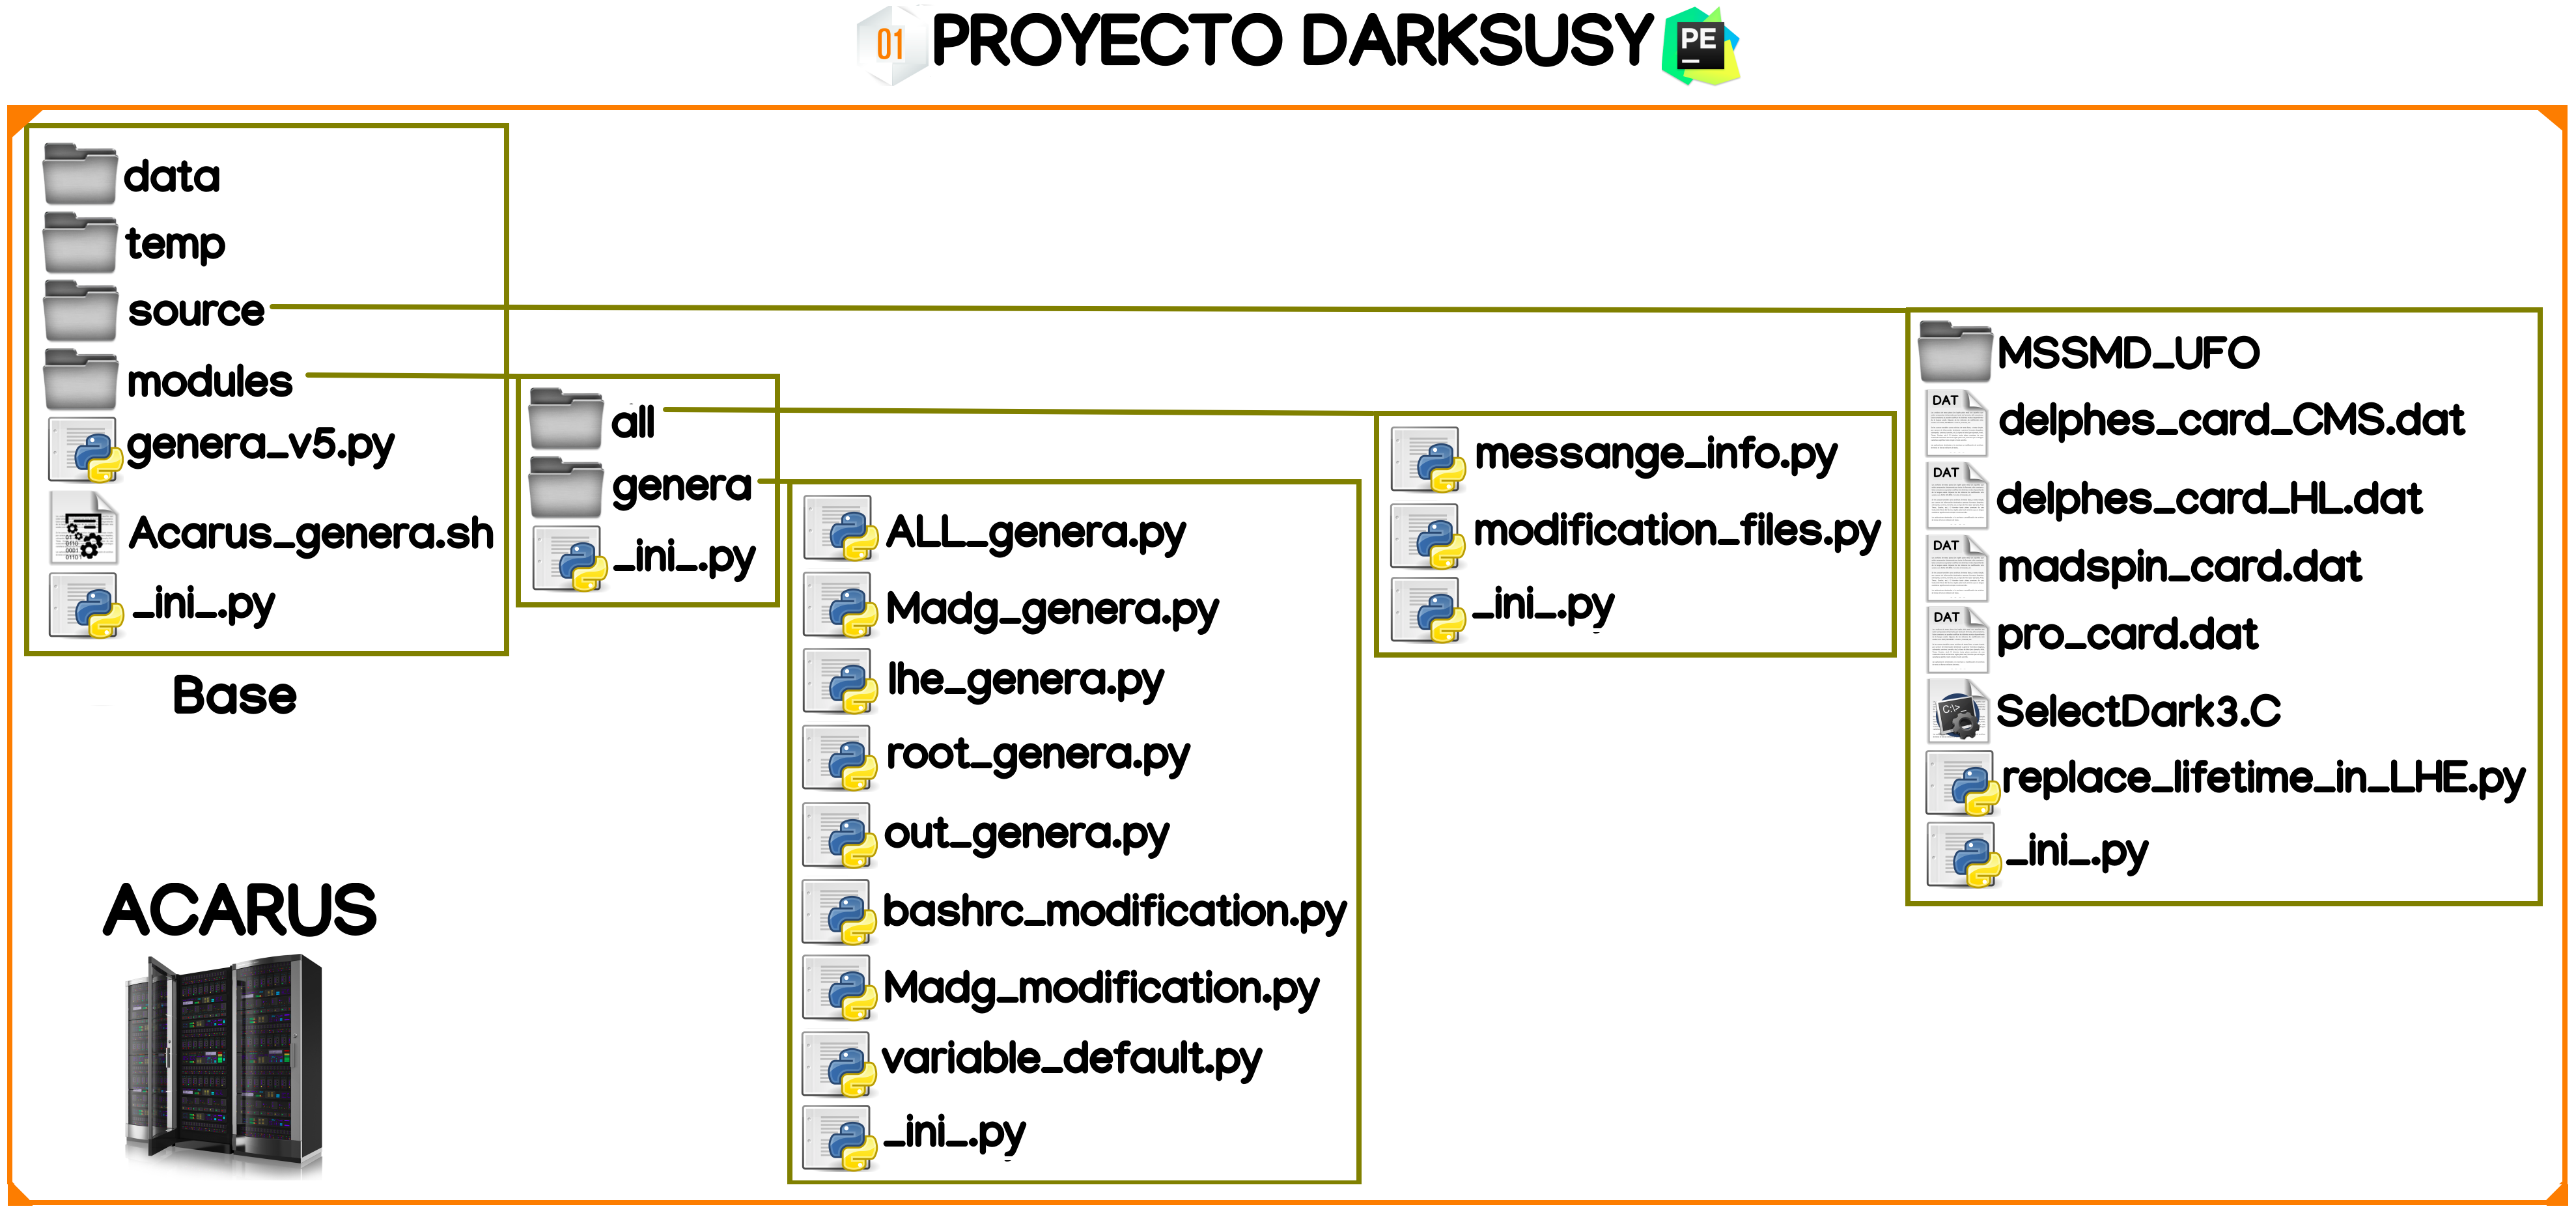
\includegraphics[width=.9\textwidth]{Simulacion/imagenes/proyecto_darksusy.png}
\caption[Estructura del proyecto de generación.]{Estructura del proyecto de generación. Página del proyecto \url{https://github.com/franky8939/GeneradorDarkSUSY}}
\label{genera_darksusy0}
\end{figure}
Ante la necesidad de flexibilizar la generación de eventos de decaimiento característicos de la Fig. \ref{fig:sketch_darksector} se crea un proyecto de programación con la capacidad de generar eventos en Madgraph bajo la variación de las masas de las partículas $n_1$ (neutralino ligero, también referido como \texttt{NeuL}), $n_D$ (neutralino oscuro, también referido como \texttt{NeuD}) y $\gamma_D$ (fotón oscuro, también referido como \texttt{PhoD}) y del tiempo de vida del último (\texttt{TcPhoD}), además de generar la simulación bajo condiciones del detector en Run-2 (referenciada en el trabajo como \texttt{CMS}) y High Luminosity (referenciada como \texttt{HL}). La estructura del proyecto se puede observar en la Fig. \ref{genera_darksusy0}.

Además para hacer uso eficiente de los recursos puestos a disposición, el proyecto creado en \texttt{python}, fue programado con la intencionalidad de automatizar la configuración necesarias para su correcta ejecución, automatizando el cambio de los parámetros de generación posteriormente definidos, inclusión del modelo \textbf{MSSMD} dentro de Madgraph y guardado automático de los resultados en un archivo externo predefinido, el flujo general del programa se puede observar en la Fig. \ref{genera_darksusy2}.

El elemento iniciador se encuentra en la función \texttt{genera\_v5.py} versión 5, con este se incluye una descripción de opciones que hacen que sea adaptable ante situaciones alternativas a su configuración original:

\texttt{
\begin{tabular}{ll}
genera\_v5.py [-h] & [-Event EVENT] [-MNeuD MNEUD] [-MNeuD MNEUD]\\
& [-MPhoD MPHOD] [-TcPhoD TCPHOD] [-Mode MODE]\\
& [-Card CARD] [-Name NAME] [-Dir\_Madg DIR\_MADG]\\
& [-Dir\_temp\_Madg DIR\_TEMP\_MADG] \\
& [-Dir\_Source DIR\_SOURCE] [-Dir\_Out DIR\_OUT]\\
\end{tabular}}\\[.4cm]
\texttt{
\begin{tabular}{ll}
optional arguments:&\\
-h, --help & Show this help message and exit\\
-Event EVENT & Number of Event\\
-MNeuD MNEUD & Mass of the Dark Neutralino\\
-MNeuL MNEUL & Mass of the Lightest Neutalino\\
-MPhoD MPHOD & Mass of the Dark Photon\\
-TcPhoD TCPHOD & Life time of the Dark Photon\\
-Mode MODE & Condition using ``in'' or ``out''\\
-Card CARD & Card using ``CMS'' or ``HL''\\
-Name NAME & Name of root file out\\
-Dir\_Madg DIR\_MADG & Directory of Madgraph\\
-Dir\_temp\_Madg DIR\_TEMP\_MADG & Directory of temporal install Madgraph\\
-Dir\_Source DIR\_SOURCE & Directory where source stay\\
-Dir\_Out DIR\_OUT & Directory of result\\
\end{tabular}}

En el directorio base (Fig. \ref{genera_darksusy0}) la carpeta \texttt{data} es donde se guardarán los resultados de la simulación, esta puede modificarse con la variable \texttt{-Dir\_Out}, lo mismo ocurre con las otras variables relacionadas con directorios. Además se permite numerosas entradas de posibles variables de los elementos de masa y tiempo de vida en forma de vectores, el programa se adaptará a todas las posibles combinaciones incluidas. 

\begin{figure}
\centering
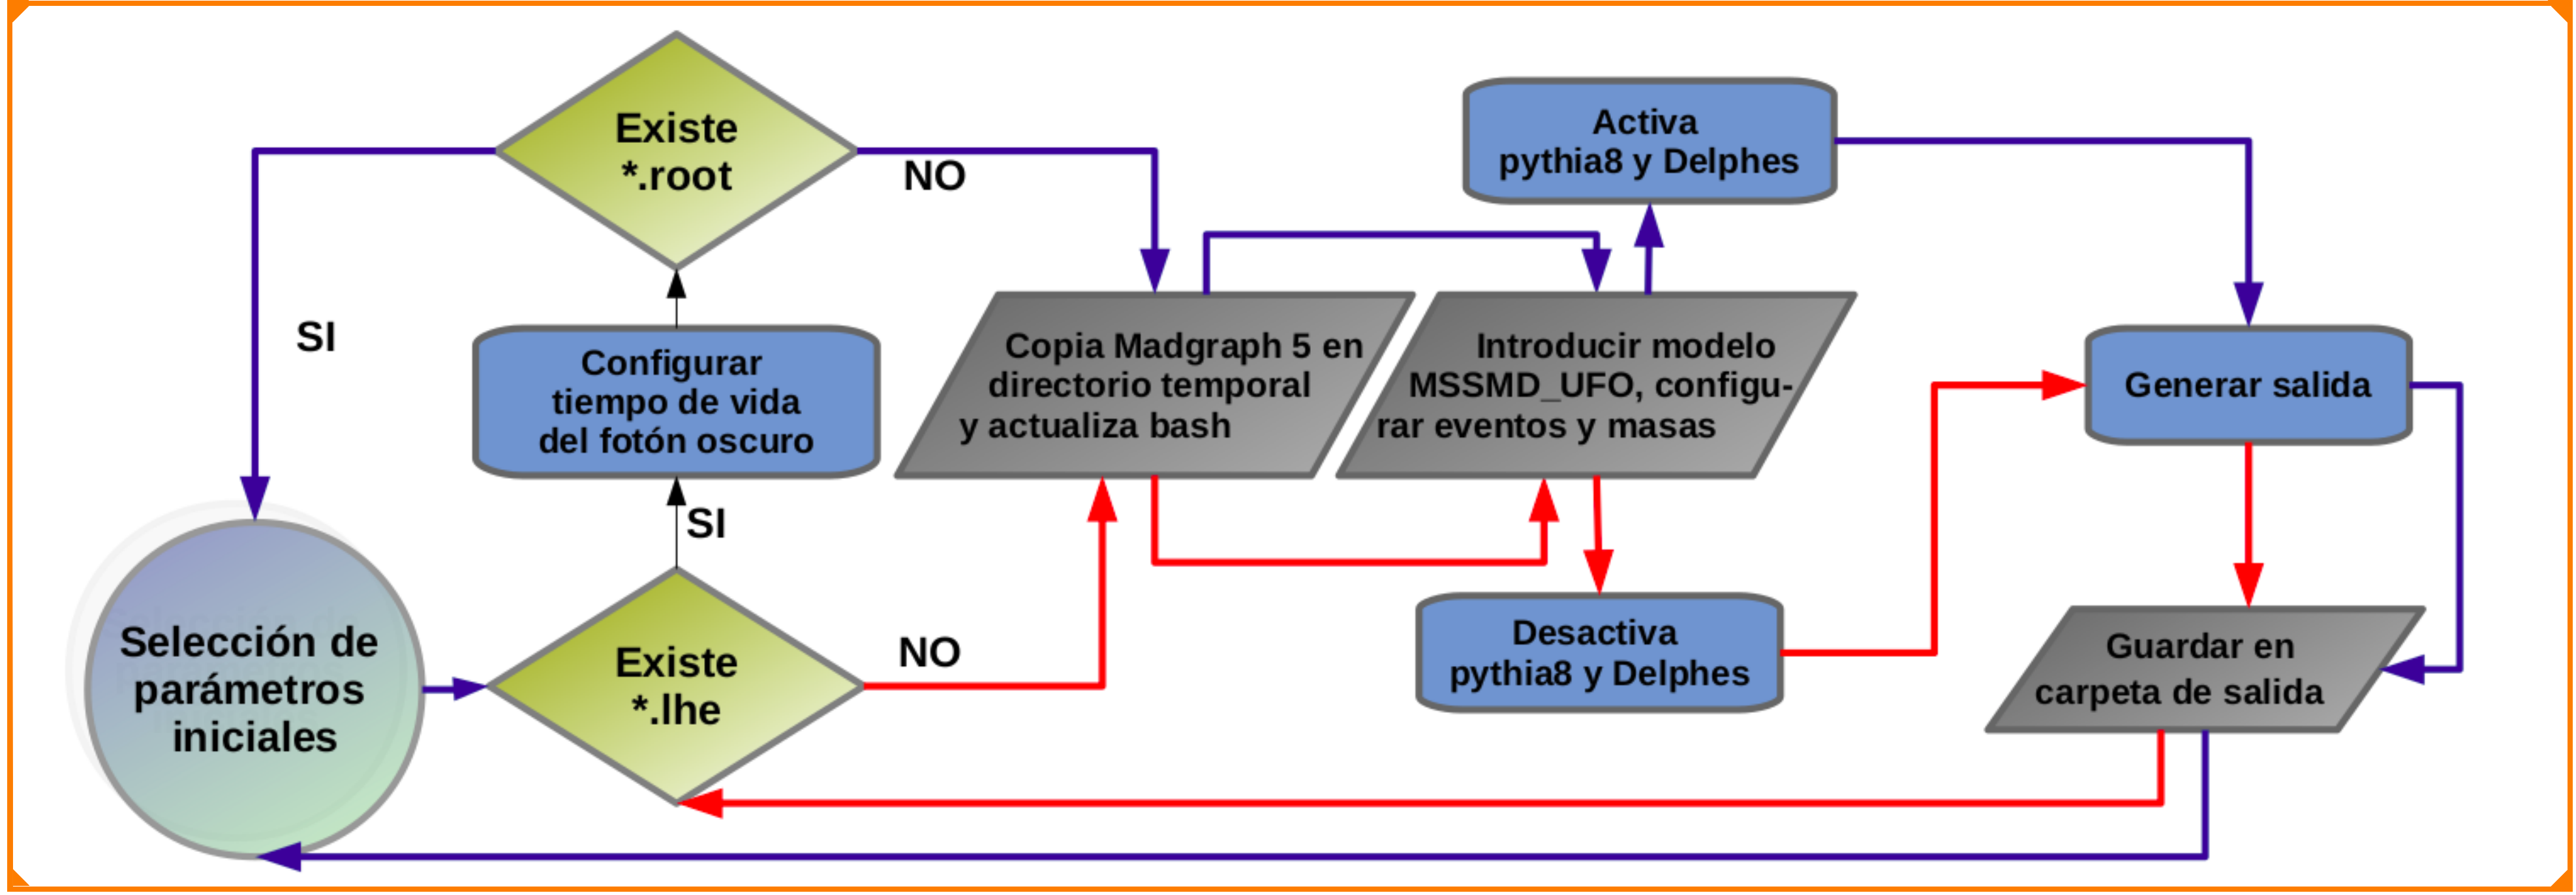
\includegraphics[width=.9\textwidth]{Simulacion/imagenes/proyecto_darksusy2.png}
\caption{Diagrama de flujo de programación del proyecto de generación.}
\label{genera_darksusy2}
\end{figure}

Es importante tener en cuenta que los archivos de monte carlo generados por MadGraph con extensión $*.lhe$ se generan para diferentes condiciones de masa (\texttt{MNeuL}, \texttt{MNeuD} y \texttt{MPhoD}), cuando  es requerido, en estos se adaptada el tiempo de vida del fotón oscuro \texttt{TcPhoD} con la función \texttt{replace\_lifetime\_in\_LHE.py}, continuando con la implementación de la herramienta de hadronización \textbf{pythia8} y por el simulador del detector \textbf{Delphes}, este último bajo las dos condiciones de configuración requeridas (Run-2 y Alta Luminosidad), de esta forma la estadística de comparación en la investigación se puede enfocar en las variaciones de las reconstrucciones del detector desechando el error por cambios de las condiciones iniciales dadas por el método \MC. 
Por defecto y por motivos de exploración básica se definen variables inicializadoras en el archivo \texttt{variable\_default.py}, estas se volverán las muestras de esta investigación:
\texttt{
\begin{tabular}{ll}
MNeuL & = $[10, ~20, ~30, ~40, ~50, ~60, ~70, ~80, ~90, ~100]$\\
Card & = [``CMS'', ``HL'']\\
MNeuD & = $[.25, ~1, ~2, ~3, ~4, ~5, ~10]$\\
MPhoD & = $[.25, ~1, ~2, ~3, ~4, ~5, ~6, ~7, ~8, ~9, ~10]$\\
TcPhoD & = $[0, ~1, ~2, ~3, ~4, ~5, ~10, ~20, ~30, ~40, ~50, ~100]$\\
Event & = 10000\\
\end{tabular}}

Como se puede observar el valor predeterminado de generación \texttt{Event} es relativamente bajo para los requerimientos de una investigación riburosa, pero será suficiente por cuando es por motivo de exploración, el tamaño de los archivos de muestras es de $\backsim$ \texttt{800 MB}, además por una cuestión de espacio la información de los eventos para valores de \texttt{Ma\_LNeu > 10} se reduce para aquellos poseedores de mínimo 4 muones. La base de datos generada para propósitos de esta investigación es de $\backsim ~2$ Terasbyte.

Para hacer referencia a los eventos definimos $\mathbb{E}_i^{(j,~k)} ~ = ~1$ donde $i = \{1, \ldots, i_{max}\}$ corresponde al elemento del evento requerido, $j = \{0\mu, ~1\mu, ~2\mu, ~3\mu, ~4\mu\, \ldots\}$ hace referencia al contenido muónico de la información por evento y $k = \{\mathtt{CMS},~\mathtt{HL}\}$ referencia al detector que generó los datos, de esta notación podemos derivar que:
\begin{equation}
\mathbb{E}^{(j,~\mathtt{CMS})} = \sum_i \mathbb{E}_i^{(j, ~\mathtt{CMS})} , ~~~~ \mathbb{E}_i^{(\mathtt{CMS})} = \sum_j \mathbb{E}_i^{(j,~\mathtt{CMS})} ~~~~ y ~~~~ \mathbb{E}^{(\mathtt{CMS})}= \sum_{ij} \mathbb{E}_i^{(j,~\mathtt{CMS})}
\end{equation}
\begin{equation}
\mathbb{E}^{(j,~\mathtt{HL})} = \sum_i \mathbb{E}_i^{(j, ~\mathtt{HL})} , ~~~~ \mathbb{E}_i^{(\mathtt{HL})} = \sum_j \mathbb{E}_i^{(j,~\mathtt{HL})} ~~~~ y ~~~~ \mathbb{E}^{(\mathtt{HL})}= \sum_{ij} \mathbb{E}_i^{(j,~\mathtt{HL})}
\end{equation}
De forma general tenemos que cada evento generado depende de las tres masas anteriormente referidas y del tiempo de vida del fotón oscuro:
\begin{equation}
\mathbb{E}_i^{(j,~k)} \equiv \mathbb{E}_i^{(j,~k)}\mathtt{(MNeuL,~MNeuD,~MPhoD,~TcPhoD)}
\end{equation}
Esta notación será la utilizada cuando se haga referencia a la información en la base de datos.




















